\documentclass[1p]{elsarticle_modified}
%\bibliographystyle{elsarticle-num}

%\usepackage[colorlinks]{hyperref}
%\usepackage{abbrmath_seonhwa} %\Abb, \Ascr, \Acal ,\Abf, \Afrak
\usepackage{amsfonts}
\usepackage{amssymb}
\usepackage{amsmath}
\usepackage{amsthm}
\usepackage{scalefnt}
\usepackage{amsbsy}
\usepackage{kotex}
\usepackage{caption}
\usepackage{subfig}
\usepackage{color}
\usepackage{graphicx}
\usepackage{xcolor} %% white, black, red, green, blue, cyan, magenta, yellow
\usepackage{float}
\usepackage{setspace}
\usepackage{hyperref}

\usepackage{tikz}
\usetikzlibrary{arrows}

\usepackage{multirow}
\usepackage{array} % fixed length table
\usepackage{hhline}

%%%%%%%%%%%%%%%%%%%%%
\makeatletter
\renewcommand*\env@matrix[1][\arraystretch]{%
	\edef\arraystretch{#1}%
	\hskip -\arraycolsep
	\let\@ifnextchar\new@ifnextchar
	\array{*\c@MaxMatrixCols c}}
\makeatother %https://tex.stackexchange.com/questions/14071/how-can-i-increase-the-line-spacing-in-a-matrix
%%%%%%%%%%%%%%%

\usepackage[normalem]{ulem}

\newcommand{\msout}[1]{\ifmmode\text{\sout{\ensuremath{#1}}}\else\sout{#1}\fi}
%SOURCE: \msout is \stkout macro in https://tex.stackexchange.com/questions/20609/strikeout-in-math-mode

\newcommand{\cancel}[1]{
	\ifmmode
	{\color{red}\msout{#1}}
	\else
	{\color{red}\sout{#1}}
	\fi
}

\newcommand{\add}[1]{
	{\color{blue}\uwave{#1}}
}

\newcommand{\replace}[2]{
	\ifmmode
	{\color{red}\msout{#1}}{\color{blue}\uwave{#2}}
	\else
	{\color{red}\sout{#1}}{\color{blue}\uwave{#2}}
	\fi
}

\newcommand{\Sol}{\mathcal{S}} %segment
\newcommand{\D}{D} %diagram
\newcommand{\A}{\mathcal{A}} %arc


%%%%%%%%%%%%%%%%%%%%%%%%%%%%%5 test

\def\sl{\operatorname{\textup{SL}}(2,\Cbb)}
\def\psl{\operatorname{\textup{PSL}}(2,\Cbb)}
\def\quan{\mkern 1mu \triangleright \mkern 1mu}

\theoremstyle{definition}
\newtheorem{thm}{Theorem}[section]
\newtheorem{prop}[thm]{Proposition}
\newtheorem{lem}[thm]{Lemma}
\newtheorem{ques}[thm]{Question}
\newtheorem{cor}[thm]{Corollary}
\newtheorem{defn}[thm]{Definition}
\newtheorem{exam}[thm]{Example}
\newtheorem{rmk}[thm]{Remark}
\newtheorem{alg}[thm]{Algorithm}

\newcommand{\I}{\sqrt{-1}}
\begin{document}

%\begin{frontmatter}
%
%\title{Boundary parabolic representations of knots up to 8 crossings}
%
%%% Group authors per affiliation:
%\author{Yunhi Cho} 
%\address{Department of Mathematics, University of Seoul, Seoul, Korea}
%\ead{yhcho@uos.ac.kr}
%
%
%\author{Seonhwa Kim} %\fnref{s_kim}}
%\address{Center for Geometry and Physics, Institute for Basic Science, Pohang, 37673, Korea}
%\ead{ryeona17@ibs.re.kr}
%
%\author{Hyuk Kim}
%\address{Department of Mathematical Sciences, Seoul National University, Seoul 08826, Korea}
%\ead{hyukkim@snu.ac.kr}
%
%\author{Seokbeom Yoon}
%\address{Department of Mathematical Sciences, Seoul National University, Seoul, 08826,  Korea}
%\ead{sbyoon15@snu.ac.kr}
%
%\begin{abstract}
%We find all boundary parabolic representation of knots up to 8 crossings.
%
%\end{abstract}
%\begin{keyword}
%    \MSC[2010] 57M25 
%\end{keyword}
%
%\end{frontmatter}

%\linenumbers
%\tableofcontents
%
\newcommand\colored[1]{\textcolor{white}{\rule[-0.35ex]{0.8em}{1.4ex}}\kern-0.8em\color{red} #1}%
%\newcommand\colored[1]{\textcolor{white}{ #1}\kern-2.17ex	\textcolor{white}{ #1}\kern-1.81ex	\textcolor{white}{ #1}\kern-2.15ex\color{red}#1	}

{\Large $\underline{11n_{4}~(K11n_{4})}$}

\setlength{\tabcolsep}{10pt}
\renewcommand{\arraystretch}{1.6}
\vspace{1cm}\begin{tabular}{m{100pt}>{\centering\arraybackslash}m{274pt}}
\multirow{5}{120pt}{
	\centering
	\includegraphics[width=112pt]{../../../GIT/diagram.site/Diagrams/png/620_11n_4.png}\\
\ \ \ A knot diagram\footnotemark}&
\allowdisplaybreaks
\textbf{Linearized knot diagam} \\
\cline{2-2}
 &
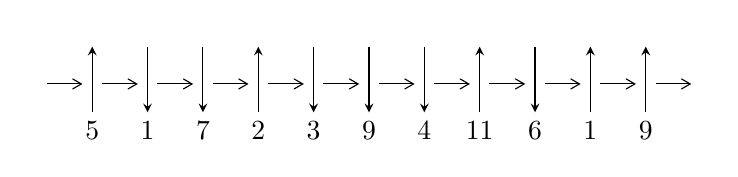
\begin{tikzpicture}[x=20pt, y=17pt]
	% nodes
	\node (C0) at (0, 0) {};
	\node (C1) at (1, 0) {};
	\node (C1U) at (1, +1) {};
	\node (C1D) at (1, -1) {5};

	\node (C2) at (2, 0) {};
	\node (C2U) at (2, +1) {};
	\node (C2D) at (2, -1) {1};

	\node (C3) at (3, 0) {};
	\node (C3U) at (3, +1) {};
	\node (C3D) at (3, -1) {7};

	\node (C4) at (4, 0) {};
	\node (C4U) at (4, +1) {};
	\node (C4D) at (4, -1) {2};

	\node (C5) at (5, 0) {};
	\node (C5U) at (5, +1) {};
	\node (C5D) at (5, -1) {3};

	\node (C6) at (6, 0) {};
	\node (C6U) at (6, +1) {};
	\node (C6D) at (6, -1) {9};

	\node (C7) at (7, 0) {};
	\node (C7U) at (7, +1) {};
	\node (C7D) at (7, -1) {4};

	\node (C8) at (8, 0) {};
	\node (C8U) at (8, +1) {};
	\node (C8D) at (8, -1) {11};

	\node (C9) at (9, 0) {};
	\node (C9U) at (9, +1) {};
	\node (C9D) at (9, -1) {6};

	\node (C10) at (10, 0) {};
	\node (C10U) at (10, +1) {};
	\node (C10D) at (10, -1) {1};

	\node (C11) at (11, 0) {};
	\node (C11U) at (11, +1) {};
	\node (C11D) at (11, -1) {9};
	\node (C12) at (12, 0) {};

	% arrows
	\draw[->,>={angle 60}]
	(C0) edge (C1) (C1) edge (C2) (C2) edge (C3) (C3) edge (C4) (C4) edge (C5) (C5) edge (C6) (C6) edge (C7) (C7) edge (C8) (C8) edge (C9) (C9) edge (C10) (C10) edge (C11) (C11) edge (C12) ;	\draw[->,>=stealth]
	(C1D) edge (C1U) (C2U) edge (C2D) (C3U) edge (C3D) (C4D) edge (C4U) (C5U) edge (C5D) (C6U) edge (C6D) (C7U) edge (C7D) (C8D) edge (C8U) (C9U) edge (C9D) (C10D) edge (C10U) (C11D) edge (C11U) ;
	\end{tikzpicture} \\
\hhline{~~} \\& 
\textbf{Solving Sequence} \\ \cline{2-2} 
 &
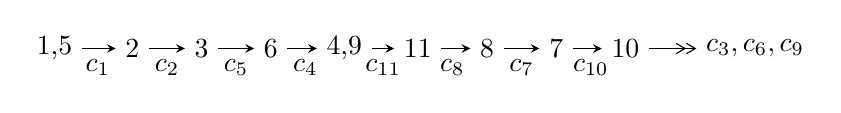
\begin{tikzpicture}[x=25pt, y=7pt]
	% node
	\node (A0) at (-1/8, 0) {1,5};
	\node (A1) at (1, 0) {2};
	\node (A2) at (2, 0) {3};
	\node (A3) at (3, 0) {6};
	\node (A4) at (65/16, 0) {4,9};
	\node (A5) at (41/8, 0) {11};
	\node (A6) at (49/8, 0) {8};
	\node (A7) at (57/8, 0) {7};
	\node (A8) at (65/8, 0) {10};
	\node (C1) at (1/2, -1) {$c_{1}$};
	\node (C2) at (3/2, -1) {$c_{2}$};
	\node (C3) at (5/2, -1) {$c_{5}$};
	\node (C4) at (7/2, -1) {$c_{4}$};
	\node (C5) at (37/8, -1) {$c_{11}$};
	\node (C6) at (45/8, -1) {$c_{8}$};
	\node (C7) at (53/8, -1) {$c_{7}$};
	\node (C8) at (61/8, -1) {$c_{10}$};
	\node (A9) at (10, 0) {$c_{3},c_{6},c_{9}$};

	% edge
	\draw[->,>=stealth]	
	(A0) edge (A1) (A1) edge (A2) (A2) edge (A3) (A3) edge (A4) (A4) edge (A5) (A5) edge (A6) (A6) edge (A7) (A7) edge (A8) ;
	\draw[->>,>={angle 60}]	
	(A8) edge (A9);
\end{tikzpicture} \\ 

\end{tabular} \\

\footnotetext{
The image of knot diagram is generated by the software ``\textbf{Draw programme}" developed by Andrew Bartholomew(\url{http://www.layer8.co.uk/maths/draw/index.htm\#Running-draw}), where we modified some parts for our purpose(\url{https://github.com/CATsTAILs/LinksPainter}).
}\phantom \\ \newline 
\centering \textbf{Ideals for irreducible components\footnotemark of $X_{\text{par}}$} 
 
\begin{align*}
I^u_{1}&=\langle 
9579649 u^{28}+28051230 u^{27}+\cdots+44628149 b-26156718,\\
\phantom{I^u_{1}}&\phantom{= \langle  }-402165 u^{28}-18012803 u^{27}+\cdots+44628149 a-25970340,\;u^{29}+2 u^{28}+\cdots- u+1\rangle \\
I^u_{2}&=\langle 
b-1,\;u^4- u^3+2 u^2+a- u+1,\;u^5- u^4+2 u^3- u^2+u-1\rangle \\
\\
\end{align*}
\raggedright * 2 irreducible components of $\dim_{\mathbb{C}}=0$, with total 34 representations.\\
\footnotetext{All coefficients of polynomials are rational numbers. But the coefficients are sometimes approximated in decimal forms when there is not enough margin.}
\newpage
\renewcommand{\arraystretch}{1}
\centering \section*{I. $I^u_{1}= \langle 9.58\times10^{6} u^{28}+2.81\times10^{7} u^{27}+\cdots+4.46\times10^{7} b-2.62\times10^{7},\;-4.02\times10^{5} u^{28}-1.80\times10^{7} u^{27}+\cdots+4.46\times10^{7} a-2.60\times10^{7},\;u^{29}+2 u^{28}+\cdots- u+1 \rangle$}
\flushleft \textbf{(i) Arc colorings}\\
\begin{tabular}{m{7pt} m{180pt} m{7pt} m{180pt} }
\flushright $a_{1}=$&$\begin{pmatrix}1\\0\end{pmatrix}$ \\
\flushright $a_{5}=$&$\begin{pmatrix}0\\u\end{pmatrix}$ \\
\flushright $a_{2}=$&$\begin{pmatrix}1\\- u^2\end{pmatrix}$ \\
\flushright $a_{3}=$&$\begin{pmatrix}u^2+1\\- u^2\end{pmatrix}$ \\
\flushright $a_{6}=$&$\begin{pmatrix}- u^5-2 u^3- u\\u^5+u^3+u\end{pmatrix}$ \\
\flushright $a_{4}=$&$\begin{pmatrix}- u\\u^3+u\end{pmatrix}$ \\
\flushright $a_{9}=$&$\begin{pmatrix}0.00901146 u^{28}+0.403620 u^{27}+\cdots+0.0183714 u+0.581927\\-0.214655 u^{28}-0.628555 u^{27}+\cdots+0.800456 u+0.586104\end{pmatrix}$ \\
\flushright $a_{11}=$&$\begin{pmatrix}-0.250701 u^{28}-0.243034 u^{27}+\cdots+0.726970 u+1.25839\\-0.141381 u^{28}-0.485781 u^{27}+\cdots+0.798176 u+0.655586\end{pmatrix}$ \\
\flushright $a_{8}=$&$\begin{pmatrix}1.26592 u^{28}+2.07814 u^{27}+\cdots-1.78235 u-0.0609626\\-0.853451 u^{28}-1.71445 u^{27}+\cdots+0.995441 u-0.861036\end{pmatrix}$ \\
\flushright $a_{7}=$&$\begin{pmatrix}0.667701 u^{28}+1.07191 u^{27}+\cdots-2.17896 u-0.0640826\\-0.263489 u^{28}-0.531459 u^{27}+\cdots+0.603619 u-0.667701\end{pmatrix}$ \\
\flushright $a_{10}=$&$\begin{pmatrix}-0.109320 u^{28}+0.242748 u^{27}+\cdots-0.0712062 u+0.602809\\-0.141381 u^{28}-0.485781 u^{27}+\cdots+0.798176 u+0.655586\end{pmatrix}$\\ \flushright $a_{10}=$&$\begin{pmatrix}-0.109320 u^{28}+0.242748 u^{27}+\cdots-0.0712062 u+0.602809\\-0.141381 u^{28}-0.485781 u^{27}+\cdots+0.798176 u+0.655586\end{pmatrix}$\\&\end{tabular}
\flushleft \textbf{(ii) Obstruction class $= -1$}\\~\\
\flushleft \textbf{(iii) Cusp Shapes $= -\frac{2569949}{44628149} u^{28}-\frac{167545923}{44628149} u^{27}+\cdots-\frac{46388860}{44628149} u+\frac{58164951}{44628149}$}\\~\\
\newpage\renewcommand{\arraystretch}{1}
\flushleft \textbf{(iv) u-Polynomials at the component}\newline \\
\begin{tabular}{m{50pt}|m{274pt}}
Crossings & \hspace{64pt}u-Polynomials at each crossing \\
\hline $$\begin{aligned}c_{1},c_{4}\end{aligned}$$&$\begin{aligned}
&u^{29}+2 u^{28}+\cdots- u+1
\end{aligned}$\\
\hline $$\begin{aligned}c_{2}\end{aligned}$$&$\begin{aligned}
&u^{29}+12 u^{28}+\cdots-5 u-1
\end{aligned}$\\
\hline $$\begin{aligned}c_{3},c_{7}\end{aligned}$$&$\begin{aligned}
&u^{29}+2 u^{28}+\cdots+u+1
\end{aligned}$\\
\hline $$\begin{aligned}c_{5}\end{aligned}$$&$\begin{aligned}
&u^{29}-2 u^{28}+\cdots-65 u+17
\end{aligned}$\\
\hline $$\begin{aligned}c_{6},c_{9}\end{aligned}$$&$\begin{aligned}
&u^{29}-5 u^{28}+\cdots+24 u^2+32
\end{aligned}$\\
\hline $$\begin{aligned}c_{8},c_{11}\end{aligned}$$&$\begin{aligned}
&u^{29}+6 u^{28}+\cdots+5 u+1
\end{aligned}$\\
\hline $$\begin{aligned}c_{10}\end{aligned}$$&$\begin{aligned}
&u^{29}-36 u^{28}+\cdots-183 u-1
\end{aligned}$\\
\hline
\end{tabular}\\~\\
\newpage\renewcommand{\arraystretch}{1}
\flushleft \textbf{(v) Riley Polynomials at the component}\newline \\
\begin{tabular}{m{50pt}|m{274pt}}
Crossings & \hspace{64pt}Riley Polynomials at each crossing \\
\hline $$\begin{aligned}c_{1},c_{4}\end{aligned}$$&$\begin{aligned}
&y^{29}+12 y^{28}+\cdots-5 y-1
\end{aligned}$\\
\hline $$\begin{aligned}c_{2}\end{aligned}$$&$\begin{aligned}
&y^{29}+12 y^{28}+\cdots-89 y-1
\end{aligned}$\\
\hline $$\begin{aligned}c_{3},c_{7}\end{aligned}$$&$\begin{aligned}
&y^{29}+30 y^{27}+\cdots-5 y-1
\end{aligned}$\\
\hline $$\begin{aligned}c_{5}\end{aligned}$$&$\begin{aligned}
&y^{29}+12 y^{28}+\cdots-13285 y-289
\end{aligned}$\\
\hline $$\begin{aligned}c_{6},c_{9}\end{aligned}$$&$\begin{aligned}
&y^{29}+33 y^{28}+\cdots-1536 y-1024
\end{aligned}$\\
\hline $$\begin{aligned}c_{8},c_{11}\end{aligned}$$&$\begin{aligned}
&y^{29}-36 y^{28}+\cdots-183 y-1
\end{aligned}$\\
\hline $$\begin{aligned}c_{10}\end{aligned}$$&$\begin{aligned}
&y^{29}-80 y^{28}+\cdots+16377 y-1
\end{aligned}$\\
\hline
\end{tabular}\\~\\
\newpage\flushleft \textbf{(vi) Complex Volumes and Cusp Shapes}
$$\begin{array}{c|c|c}  
\text{Solutions to }I^u_{1}& \I (\text{vol} + \sqrt{-1}CS) & \text{Cusp shape}\\
 \hline 
\begin{aligned}
u &= \phantom{-}0.387233 + 0.859940 I \\
a &= \phantom{-}0.839842 - 0.200433 I \\
b &= -0.0183680 - 0.0952600 I\end{aligned}
 & -0.34137 + 1.65783 I & -2.51721 - 4.37356 I \\ \hline\begin{aligned}
u &= \phantom{-}0.387233 - 0.859940 I \\
a &= \phantom{-}0.839842 + 0.200433 I \\
b &= -0.0183680 + 0.0952600 I\end{aligned}
 & -0.34137 - 1.65783 I & -2.51721 + 4.37356 I \\ \hline\begin{aligned}
u &= \phantom{-}0.525029 + 0.781903 I \\
a &= -1.45815 - 1.69363 I \\
b &= \phantom{-}0.960834 - 0.144408 I\end{aligned}
 & \phantom{-}1.78487 + 1.57609 I & \phantom{-}0.9666 - 16.5900 I \\ \hline\begin{aligned}
u &= \phantom{-}0.525029 - 0.781903 I \\
a &= -1.45815 + 1.69363 I \\
b &= \phantom{-}0.960834 + 0.144408 I\end{aligned}
 & \phantom{-}1.78487 - 1.57609 I & \phantom{-}0.9666 + 16.5900 I \\ \hline\begin{aligned}
u &= -0.654583 + 0.675856 I \\
a &= -0.197062 - 0.780511 I \\
b &= \phantom{-}0.929333 + 1.022590 I\end{aligned}
 & \phantom{-}3.12622 + 1.43345 I & \phantom{-}4.04144 - 2.82912 I \\ \hline\begin{aligned}
u &= -0.654583 - 0.675856 I \\
a &= -0.197062 + 0.780511 I \\
b &= \phantom{-}0.929333 - 1.022590 I\end{aligned}
 & \phantom{-}3.12622 - 1.43345 I & \phantom{-}4.04144 + 2.82912 I \\ \hline\begin{aligned}
u &= -0.925881 + 0.518414 I \\
a &= \phantom{-}1.81441 + 0.23795 I \\
b &= -1.71997 - 0.32324 I\end{aligned}
 & \phantom{-}11.74770 + 6.59261 I & \phantom{-}3.06245 - 2.55361 I \\ \hline\begin{aligned}
u &= -0.925881 - 0.518414 I \\
a &= \phantom{-}1.81441 - 0.23795 I \\
b &= -1.71997 + 0.32324 I\end{aligned}
 & \phantom{-}11.74770 - 6.59261 I & \phantom{-}3.06245 + 2.55361 I \\ \hline\begin{aligned}
u &= \phantom{-}0.937398 + 0.500154 I \\
a &= \phantom{-}1.79802 - 0.06455 I \\
b &= -1.70627 - 0.02414 I\end{aligned}
 & \phantom{-}11.61340 + 1.70244 I & \phantom{-}3.44440 - 1.84569 I \\ \hline\begin{aligned}
u &= \phantom{-}0.937398 - 0.500154 I \\
a &= \phantom{-}1.79802 + 0.06455 I \\
b &= -1.70627 + 0.02414 I\end{aligned}
 & \phantom{-}11.61340 - 1.70244 I & \phantom{-}3.44440 + 1.84569 I\\
 \hline 
 \end{array}$$\newpage$$\begin{array}{c|c|c}  
\text{Solutions to }I^u_{1}& \I (\text{vol} + \sqrt{-1}CS) & \text{Cusp shape}\\
 \hline 
\begin{aligned}
u &= -0.662767 + 0.848656 I \\
a &= -1.81457 - 1.32278 I \\
b &= \phantom{-}1.81677 - 0.13637 I\end{aligned}
 & \phantom{-}5.01547 - 2.56835 I & \phantom{-}6.29777 + 3.45072 I \\ \hline\begin{aligned}
u &= -0.662767 - 0.848656 I \\
a &= -1.81457 + 1.32278 I \\
b &= \phantom{-}1.81677 + 0.13637 I\end{aligned}
 & \phantom{-}5.01547 + 2.56835 I & \phantom{-}6.29777 - 3.45072 I \\ \hline\begin{aligned}
u &= \phantom{-}0.567900 + 0.933831 I \\
a &= -0.28660 + 1.95388 I \\
b &= \phantom{-}0.704163 + 0.280595 I\end{aligned}
 & \phantom{-}1.23273 + 2.84215 I & \phantom{-}0.371066 + 0.581587 I \\ \hline\begin{aligned}
u &= \phantom{-}0.567900 - 0.933831 I \\
a &= -0.28660 - 1.95388 I \\
b &= \phantom{-}0.704163 - 0.280595 I\end{aligned}
 & \phantom{-}1.23273 - 2.84215 I & \phantom{-}0.371066 - 0.581587 I \\ \hline\begin{aligned}
u &= -0.043975 + 0.873551 I \\
a &= \phantom{-}1.118610 + 0.586417 I \\
b &= \phantom{-}0.157858 + 0.616140 I\end{aligned}
 & -1.21438 + 1.50101 I & -6.11641 - 3.93982 I \\ \hline\begin{aligned}
u &= -0.043975 - 0.873551 I \\
a &= \phantom{-}1.118610 - 0.586417 I \\
b &= \phantom{-}0.157858 - 0.616140 I\end{aligned}
 & -1.21438 - 1.50101 I & -6.11641 + 3.93982 I \\ \hline\begin{aligned}
u &= -0.637441 + 0.973302 I \\
a &= -1.34495 - 0.55786 I \\
b &= \phantom{-}0.69848 - 1.23040 I\end{aligned}
 & \phantom{-}2.23506 - 6.49074 I & \phantom{-}1.39267 + 8.34462 I \\ \hline\begin{aligned}
u &= -0.637441 - 0.973302 I \\
a &= -1.34495 + 0.55786 I \\
b &= \phantom{-}0.69848 + 1.23040 I\end{aligned}
 & \phantom{-}2.23506 + 6.49074 I & \phantom{-}1.39267 - 8.34462 I \\ \hline\begin{aligned}
u &= -0.461488 + 1.163620 I \\
a &= \phantom{-}0.358541 + 0.419840 I \\
b &= -0.655831 - 0.154039 I\end{aligned}
 & -4.83578 - 4.15032 I & -10.94337 + 1.86325 I \\ \hline\begin{aligned}
u &= -0.461488 - 1.163620 I \\
a &= \phantom{-}0.358541 - 0.419840 I \\
b &= -0.655831 + 0.154039 I\end{aligned}
 & -4.83578 + 4.15032 I & -10.94337 - 1.86325 I\\
 \hline 
 \end{array}$$\newpage$$\begin{array}{c|c|c}  
\text{Solutions to }I^u_{1}& \I (\text{vol} + \sqrt{-1}CS) & \text{Cusp shape}\\
 \hline 
\begin{aligned}
u &= \phantom{-}0.017652 + 1.279430 I \\
a &= -0.248173 - 0.176688 I \\
b &= -1.56169 - 0.18501 I\end{aligned}
 & \phantom{-}4.96946 + 4.25609 I & -1.11871 - 2.71437 I \\ \hline\begin{aligned}
u &= \phantom{-}0.017652 - 1.279430 I \\
a &= -0.248173 + 0.176688 I \\
b &= -1.56169 + 0.18501 I\end{aligned}
 & \phantom{-}4.96946 - 4.25609 I & -1.11871 + 2.71437 I \\ \hline\begin{aligned}
u &= -0.697556 + 1.121820 I \\
a &= \phantom{-}1.35862 + 1.61660 I \\
b &= -1.69014 + 0.41795 I\end{aligned}
 & \phantom{-}9.9003 - 12.5531 I & \phantom{-}0.87648 + 6.84593 I \\ \hline\begin{aligned}
u &= -0.697556 - 1.121820 I \\
a &= \phantom{-}1.35862 - 1.61660 I \\
b &= -1.69014 - 0.41795 I\end{aligned}
 & \phantom{-}9.9003 + 12.5531 I & \phantom{-}0.87648 - 6.84593 I \\ \hline\begin{aligned}
u &= \phantom{-}0.697068 + 1.137050 I \\
a &= \phantom{-}0.98961 - 1.53355 I \\
b &= -1.66331 - 0.08384 I\end{aligned}
 & \phantom{-}9.66493 + 4.29038 I & \phantom{-}1.47355 - 2.52385 I \\ \hline\begin{aligned}
u &= \phantom{-}0.697068 - 1.137050 I \\
a &= \phantom{-}0.98961 + 1.53355 I \\
b &= -1.66331 + 0.08384 I\end{aligned}
 & \phantom{-}9.66493 - 4.29038 I & \phantom{-}1.47355 + 2.52385 I \\ \hline\begin{aligned}
u &= -0.659229\phantom{ +0.000000I} \\
a &= \phantom{-}1.11847\phantom{ +0.000000I} \\
b &= -0.442580\phantom{ +0.000000I}\end{aligned}
 & -1.67720\phantom{ +0.000000I} & -6.86830\phantom{ +0.000000I} \\ \hline\begin{aligned}
u &= \phantom{-}0.281024 + 0.265729 I \\
a &= \phantom{-}1.012610 - 0.151234 I \\
b &= \phantom{-}0.969423 + 0.291280 I\end{aligned}
 & \phantom{-}1.86776 + 0.92254 I & \phantom{-}4.20343 - 0.65997 I \\ \hline\begin{aligned}
u &= \phantom{-}0.281024 - 0.265729 I \\
a &= \phantom{-}1.012610 + 0.151234 I \\
b &= \phantom{-}0.969423 - 0.291280 I\end{aligned}
 & \phantom{-}1.86776 - 0.92254 I & \phantom{-}4.20343 + 0.65997 I\\
 \hline 
 \end{array}$$\newpage\newpage\renewcommand{\arraystretch}{1}
\centering \section*{II. $I^u_{2}= \langle b-1,\;u^4- u^3+2 u^2+a- u+1,\;u^5- u^4+2 u^3- u^2+u-1 \rangle$}
\flushleft \textbf{(i) Arc colorings}\\
\begin{tabular}{m{7pt} m{180pt} m{7pt} m{180pt} }
\flushright $a_{1}=$&$\begin{pmatrix}1\\0\end{pmatrix}$ \\
\flushright $a_{5}=$&$\begin{pmatrix}0\\u\end{pmatrix}$ \\
\flushright $a_{2}=$&$\begin{pmatrix}1\\- u^2\end{pmatrix}$ \\
\flushright $a_{3}=$&$\begin{pmatrix}u^2+1\\- u^2\end{pmatrix}$ \\
\flushright $a_{6}=$&$\begin{pmatrix}- u^4- u^2-1\\u^4- u^3+u^2+1\end{pmatrix}$ \\
\flushright $a_{4}=$&$\begin{pmatrix}- u\\u^3+u\end{pmatrix}$ \\
\flushright $a_{9}=$&$\begin{pmatrix}- u^4+u^3-2 u^2+u-1\\1\end{pmatrix}$ \\
\flushright $a_{11}=$&$\begin{pmatrix}- u^4+u^3-2 u^2+u\\1\end{pmatrix}$ \\
\flushright $a_{8}=$&$\begin{pmatrix}-1\\0\end{pmatrix}$ \\
\flushright $a_{7}=$&$\begin{pmatrix}- u^4- u^2-1\\u^4- u^3+u^2+1\end{pmatrix}$ \\
\flushright $a_{10}=$&$\begin{pmatrix}- u^4+u^3-2 u^2+u-1\\1\end{pmatrix}$\\ \flushright $a_{10}=$&$\begin{pmatrix}- u^4+u^3-2 u^2+u-1\\1\end{pmatrix}$\\&\end{tabular}
\flushleft \textbf{(ii) Obstruction class $= 1$}\\~\\
\flushleft \textbf{(iii) Cusp Shapes $= 3 u^4+3 u^3-4 u^2+8 u-3$}\\~\\
\newpage\renewcommand{\arraystretch}{1}
\flushleft \textbf{(iv) u-Polynomials at the component}\newline \\
\begin{tabular}{m{50pt}|m{274pt}}
Crossings & \hspace{64pt}u-Polynomials at each crossing \\
\hline $$\begin{aligned}c_{1}\end{aligned}$$&$\begin{aligned}
&u^5- u^4+2 u^3- u^2+u-1
\end{aligned}$\\
\hline $$\begin{aligned}c_{2}\end{aligned}$$&$\begin{aligned}
&u^5+3 u^4+4 u^3+u^2- u-1
\end{aligned}$\\
\hline $$\begin{aligned}c_{3}\end{aligned}$$&$\begin{aligned}
&u^5+u^4-2 u^3- u^2+u-1
\end{aligned}$\\
\hline $$\begin{aligned}c_{4}\end{aligned}$$&$\begin{aligned}
&u^5+u^4+2 u^3+u^2+u+1
\end{aligned}$\\
\hline $$\begin{aligned}c_{5},c_{7}\end{aligned}$$&$\begin{aligned}
&u^5- u^4-2 u^3+u^2+u+1
\end{aligned}$\\
\hline $$\begin{aligned}c_{6},c_{9}\end{aligned}$$&$\begin{aligned}
&u^5
\end{aligned}$\\
\hline $$\begin{aligned}c_{8},c_{10}\end{aligned}$$&$\begin{aligned}
&(u+1)^5
\end{aligned}$\\
\hline $$\begin{aligned}c_{11}\end{aligned}$$&$\begin{aligned}
&(u-1)^5
\end{aligned}$\\
\hline
\end{tabular}\\~\\
\newpage\renewcommand{\arraystretch}{1}
\flushleft \textbf{(v) Riley Polynomials at the component}\newline \\
\begin{tabular}{m{50pt}|m{274pt}}
Crossings & \hspace{64pt}Riley Polynomials at each crossing \\
\hline $$\begin{aligned}c_{1},c_{4}\end{aligned}$$&$\begin{aligned}
&y^5+3 y^4+4 y^3+y^2- y-1
\end{aligned}$\\
\hline $$\begin{aligned}c_{2}\end{aligned}$$&$\begin{aligned}
&y^5- y^4+8 y^3-3 y^2+3 y-1
\end{aligned}$\\
\hline $$\begin{aligned}c_{3},c_{5},c_{7}\end{aligned}$$&$\begin{aligned}
&y^5-5 y^4+8 y^3-3 y^2- y-1
\end{aligned}$\\
\hline $$\begin{aligned}c_{6},c_{9}\end{aligned}$$&$\begin{aligned}
&y^5
\end{aligned}$\\
\hline $$\begin{aligned}c_{8},c_{10},c_{11}\end{aligned}$$&$\begin{aligned}
&(y-1)^5
\end{aligned}$\\
\hline
\end{tabular}\\~\\
\newpage\flushleft \textbf{(vi) Complex Volumes and Cusp Shapes}
$$\begin{array}{c|c|c}  
\text{Solutions to }I^u_{2}& \I (\text{vol} + \sqrt{-1}CS) & \text{Cusp shape}\\
 \hline 
\begin{aligned}
u &= -0.339110 + 0.822375 I \\
a &= \phantom{-}0.428550 + 1.039280 I \\
b &= \phantom{-}1.00000\phantom{ +0.000000I}\end{aligned}
 & \phantom{-}1.31583 - 1.53058 I & -1.50865 + 9.87103 I \\ \hline\begin{aligned}
u &= -0.339110 - 0.822375 I \\
a &= \phantom{-}0.428550 - 1.039280 I \\
b &= \phantom{-}1.00000\phantom{ +0.000000I}\end{aligned}
 & \phantom{-}1.31583 + 1.53058 I & -1.50865 - 9.87103 I \\ \hline\begin{aligned}
u &= \phantom{-}0.766826\phantom{ +0.000000I} \\
a &= -1.30408\phantom{ +0.000000I} \\
b &= \phantom{-}1.00000\phantom{ +0.000000I}\end{aligned}
 & -0.756147\phantom{ +0.000000I} & \phantom{-}3.17260\phantom{ +0.000000I} \\ \hline\begin{aligned}
u &= \phantom{-}0.455697 + 1.200150 I \\
a &= -0.276511 + 0.728237 I \\
b &= \phantom{-}1.00000\phantom{ +0.000000I}\end{aligned}
 & -4.22763 + 4.40083 I & \phantom{-}0.92237 - 5.80708 I \\ \hline\begin{aligned}
u &= \phantom{-}0.455697 - 1.200150 I \\
a &= -0.276511 - 0.728237 I \\
b &= \phantom{-}1.00000\phantom{ +0.000000I}\end{aligned}
 & -4.22763 - 4.40083 I & \phantom{-}0.92237 + 5.80708 I\\
 \hline 
 \end{array}$$\newpage
\newpage\renewcommand{\arraystretch}{1}
\centering \section*{ III. u-Polynomials}
\begin{tabular}{m{50pt}|m{274pt}}
Crossings & \hspace{64pt}u-Polynomials at each crossing \\
\hline $$\begin{aligned}c_{1}\end{aligned}$$&$\begin{aligned}
&(u^5- u^4+2 u^3- u^2+u-1)(u^{29}+2 u^{28}+\cdots- u+1)
\end{aligned}$\\
\hline $$\begin{aligned}c_{2}\end{aligned}$$&$\begin{aligned}
&(u^5+3 u^4+4 u^3+u^2- u-1)(u^{29}+12 u^{28}+\cdots-5 u-1)
\end{aligned}$\\
\hline $$\begin{aligned}c_{3}\end{aligned}$$&$\begin{aligned}
&(u^5+u^4-2 u^3- u^2+u-1)(u^{29}+2 u^{28}+\cdots+u+1)
\end{aligned}$\\
\hline $$\begin{aligned}c_{4}\end{aligned}$$&$\begin{aligned}
&(u^5+u^4+2 u^3+u^2+u+1)(u^{29}+2 u^{28}+\cdots- u+1)
\end{aligned}$\\
\hline $$\begin{aligned}c_{5}\end{aligned}$$&$\begin{aligned}
&(u^5- u^4-2 u^3+u^2+u+1)(u^{29}-2 u^{28}+\cdots-65 u+17)
\end{aligned}$\\
\hline $$\begin{aligned}c_{6},c_{9}\end{aligned}$$&$\begin{aligned}
&u^5(u^{29}-5 u^{28}+\cdots+24 u^2+32)
\end{aligned}$\\
\hline $$\begin{aligned}c_{7}\end{aligned}$$&$\begin{aligned}
&(u^5- u^4-2 u^3+u^2+u+1)(u^{29}+2 u^{28}+\cdots+u+1)
\end{aligned}$\\
\hline $$\begin{aligned}c_{8}\end{aligned}$$&$\begin{aligned}
&((u+1)^5)(u^{29}+6 u^{28}+\cdots+5 u+1)
\end{aligned}$\\
\hline $$\begin{aligned}c_{10}\end{aligned}$$&$\begin{aligned}
&((u+1)^5)(u^{29}-36 u^{28}+\cdots-183 u-1)
\end{aligned}$\\
\hline $$\begin{aligned}c_{11}\end{aligned}$$&$\begin{aligned}
&((u-1)^5)(u^{29}+6 u^{28}+\cdots+5 u+1)
\end{aligned}$\\
\hline
\end{tabular}\newpage\renewcommand{\arraystretch}{1}
\centering \section*{ IV. Riley Polynomials}
\begin{tabular}{m{50pt}|m{274pt}}
Crossings & \hspace{64pt}Riley Polynomials at each crossing \\
\hline $$\begin{aligned}c_{1},c_{4}\end{aligned}$$&$\begin{aligned}
&(y^5+3 y^4+4 y^3+y^2- y-1)(y^{29}+12 y^{28}+\cdots-5 y-1)
\end{aligned}$\\
\hline $$\begin{aligned}c_{2}\end{aligned}$$&$\begin{aligned}
&(y^5- y^4+8 y^3-3 y^2+3 y-1)(y^{29}+12 y^{28}+\cdots-89 y-1)
\end{aligned}$\\
\hline $$\begin{aligned}c_{3},c_{7}\end{aligned}$$&$\begin{aligned}
&(y^5-5 y^4+8 y^3-3 y^2- y-1)(y^{29}+30 y^{27}+\cdots-5 y-1)
\end{aligned}$\\
\hline $$\begin{aligned}c_{5}\end{aligned}$$&$\begin{aligned}
&(y^5-5 y^4+8 y^3-3 y^2- y-1)(y^{29}+12 y^{28}+\cdots-13285 y-289)
\end{aligned}$\\
\hline $$\begin{aligned}c_{6},c_{9}\end{aligned}$$&$\begin{aligned}
&y^5(y^{29}+33 y^{28}+\cdots-1536 y-1024)
\end{aligned}$\\
\hline $$\begin{aligned}c_{8},c_{11}\end{aligned}$$&$\begin{aligned}
&((y-1)^5)(y^{29}-36 y^{28}+\cdots-183 y-1)
\end{aligned}$\\
\hline $$\begin{aligned}c_{10}\end{aligned}$$&$\begin{aligned}
&((y-1)^5)(y^{29}-80 y^{28}+\cdots+16377 y-1)
\end{aligned}$\\
\hline
\end{tabular}
\vskip 2pc
\end{document}